\subsection{Results}

\subsubsection{GemNet}

We evaluated the GemNet model on the S2EF task with the 200k dataset and
the IS2RE task with the 100k dataset. For both tasks, we trained for one epoch
using a batch size of 16 (since data parallelism was activated in all of the 
runs, this implies that each of the 8 GPUs received 2 molecules per forward pass). 

We evaluated the GPU memory consumed by CUDA tensors and runtimes for GemNet training with 8 different 
configurations of DeepSpeed:
The so-called DeepSpeed ZeRO stage 0 served as baseline for evaluations, in which 
all DeepSpeed optimizations are deactivated---i.e. stage 0 corresponds to basic 
data-parallel training. As a second configuration, we trained GemNet 
in half precision without any ZeRO optimizations in order to make sure that
potential memory savings by ZeRO are actually caused by the model state partitioning and
not merely by reducing the model parameters' precision.

Apart from this, we evaluated two configurations of each stage of ZeRO-DP to benchmark 
them against the two baselines. More precisely, for stage 1, we did one run with and 
without overlapping communication each, while overlapping communication
was activated throughout stage 2 and stage 3. In order to investigate potential 
memory savings by CPU offloading, we conducted standard stage 2 and stage 3 runs as well
as runs in which the respective maximal CPU offloading ability was exploited.
The exact configurations and results can be seen in Figure~\ref{fig:gemnet-results}, 
where \enquote{OC} stands for overlapping communication,
\enquote{OO} for optimizer offloading and \enquote{PO} for parameter offloading.

\begin{figure}[H]
    \centering

    \begin{subfigure}[t]{0.48\textwidth}
        \centering
        \includegraphics[width=\textwidth]{evaluation/gemnet/s2ef/cuda_memory/memory_comparison.pdf}
    \end{subfigure}%
    ~
    \begin{subfigure}[t]{0.48\textwidth}
        \centering
        \includegraphics[width=\textwidth]{evaluation/gemnet/s2ef/runtimes/runtimes_comparison.pdf}
    \end{subfigure}

    \resizebox{0.95\textwidth}{!}{%
    \begin{tabular}{ll|l|l|l|l|l|l|l|l|}
    \cline{3-10}
    \textbf{S2EF} & & \scriptsize \textbf{S0}    & \scriptsize \textbf{S0}+fp16 & \scriptsize \textbf{S1}             & \scriptsize \textbf{S1}+OC          & \scriptsize \textbf{S2}+OC & \begin{tabular}{@{}c@{}}\scriptsize\textbf{S2}+OO \vspace*{-0.5em} \\ \scriptsize+OC\end{tabular}      & \scriptsize \textbf{S3}+OC & \scriptsize \begin{tabular}{@{}c@{}}\scriptsize\textbf{S3}+PO \\ \scriptsize+OO+OC\end{tabular} \\ \hline \hline
    \multicolumn{1}{|l|}{\multirow{2}{*}{memory}}   & allocated   & 7.11     & 7.1               & 2.36           & 2.36              & 2.36     & \textbf{1.78} & 3.51     & 2.78              \\ \cline{2-10} 
    \multicolumn{1}{|l|}{}                          & reserved    & 37.71    & 24.98             & \textbf{18.99} & \textbf{18.99}    & 20.3     & 19.77         & 21.99    & 21.32             \\ \hline \hline
    \multicolumn{1}{|l|}{\multirow{5}{*}{runtimes}} & epoch       & 04:07:00 & \textbf{02:29:03} & 02:43:45       & 02:42:51          & 03:00:41 & 04:18:11      & 03:43:01 & 05:09:53          \\ \cline{2-10} 
    \multicolumn{1}{|l|}{}                          & dataloading & 00:00:51 & 00:00:45          & 00:00:29       & 00:00:26          & 00:00:30 & 00:00:29      & 00:00:27 & \textbf{00:00:24} \\ \cline{2-10} 
    \multicolumn{1}{|l|}{}                          & forward     & 00:35:43 & \textbf{00:21:36} & 00:21:59       & 00:21:57          & 00:21:58 & 00:21:57      & 00:54:57 & 00:54:32          \\ \cline{2-10} 
    \multicolumn{1}{|l|}{}                          & backward    & 03:11:31 & 01:53:35          & 01:39:38       & \textbf{01:38:45} & 01:56:29 & 03:09:20      & 02:05:26 & 03:52:43          \\ \cline{2-10} 
    \multicolumn{1}{|l|}{}                          & rest        & 00:18:53 & \textbf{00:13:05} & 00:41:39       & 00:41:41          & 00:41:43 & 00:46:23      & 00:42:11 & 00:22:13          \\ \hline
    \end{tabular}}

    \vspace*{2em}

    \begin{subfigure}[t]{0.48\textwidth}
        \centering
        \includegraphics[width=\textwidth]{evaluation/gemnet/is2re/cuda_memory/memory_comparison.pdf}
    \end{subfigure}%
    ~
    \begin{subfigure}[t]{0.48\textwidth}
        \centering
        \includegraphics[width=\textwidth]{evaluation/gemnet/is2re/runtimes/runtimes_comparison.pdf}
    \end{subfigure}

    \resizebox{0.95\textwidth}{!}{%
    \begin{tabular}{ll|l|l|l|l|l|l|l|l|}
    \cline{3-10}
    \textbf{IS2RE} & & \scriptsize \textbf{S0}    & \scriptsize \textbf{S0}+fp16 & \scriptsize \textbf{S1}             & \scriptsize \textbf{S1}+OC          & \scriptsize \textbf{S2}+OC & \begin{tabular}{@{}c@{}}\scriptsize\textbf{S2}+OO \vspace*{-0.5em} \\ \scriptsize+OC\end{tabular}      & \scriptsize \textbf{S3}+OC & \scriptsize \begin{tabular}{@{}c@{}}\scriptsize\textbf{S3}+PO \\ \scriptsize+OO+OC\end{tabular} \\ \hline \hline
    \multicolumn{1}{|l|}{\multirow{2}{*}{memory}}   & allocated   & 2.88     & 2.88              & 0.62              & 0.62           & 0.62     & \textbf{0.36}  & 1.36              & 1.0         \\ \cline{2-10} 
    \multicolumn{1}{|l|}{}                          & reserved    & 36.27    & 20.6              & \textbf{18.19}    & \textbf{18.19} & 19.24    & \textbf{18.19} & 19.44             & 19.68       \\ \hline \hline
    \multicolumn{1}{|l|}{\multirow{5}{*}{runtimes}} & epoch       & 01:40:32 & 01:03:09          & \textbf{01:01:58} & 01:02:39       & 01:13:23 & 01:33:50       & 01:20:55          & 01:56:20    \\ \cline{2-10} 
    \multicolumn{1}{|l|}{}                          & dataloading & 00:00:09 & 00:00:13          & 00:00:09          & 00:00:09       & 00:00:08 & 00:00:11       & \textbf{00:00:07} & 00:00:15    \\ \cline{2-10} 
    \multicolumn{1}{|l|}{}                          & forward     & 00:24:17 & \textbf{00:15:43} & 00:16:07          & 00:16:06       & 00:16:04 & 00:16:07       & 00:27:31          & 00:27:30    \\ \cline{2-10} 
    \multicolumn{1}{|l|}{}                          & backward    & 01:10:58 & 00:43:16          & \textbf{00:39:29} & 00:39:35       & 00:45:34 & 01:04:43       & 00:42:51          & 01:16:32    \\ \cline{2-10} 
    \multicolumn{1}{|l|}{}                          & rest        & 00:05:07 & \textbf{00:03:55} & 00:06:12          & 00:06:47       & 00:11:35 & 00:12:47       & 00:10:25          & 00:12:01    \\ \hline
    \end{tabular}}

    \vspace*{1em}

    \captionsetup{width=\dimexpr\textwidth-1.5cm\relax}
    \caption{Memory consumption and runtimes for GemNet. 
    Memory is in GB, runtimes in the \textit{h:m:s} format.}
    \label{fig:gemnet-results}
    
\end{figure}

While enabling half precision training on stage 0 does significantly reduce 
reserved memory, allocated memory is only marginally affected. Nevertheless, 
a decrease of runtime by about 40\% (S2EF) and 41\% (IS2RE) can be observed.

When comparing stage 0 with half precision to standard stage 1, a significant decrease
both in allocated GPU memory and reserved GPU memory can be observed
(S2EF: -67\% allocated, -23\% reserved; IS2RE: -78\% allocated, -12\% reserved).
This drop in memory consumption has to be caused by optimizer state partitioning among
the GPUs since this is the only difference between the configurations. 
Both for the S2EF task and the IS2RE task, forward and backward pass 
are marginally faster with stage 1 activated. 
However, especially for the S2EF task, it is also clearly visible that communication overhead 
between the GPUs rises for stage 1: The part of the total epoch runtime which
neither belongs to one of the tracked stages (calles \enquote{rest} in 
Figure~\ref{fig:gemnet-results}) and thus mainly 
encompasses communication, increases by 219\% (S2EF) and 58\% (IS2RE).

Additionally, CPU offloading saves memory---most notable is a 58\% decrease of allocated GPU 
memory with IS2RE when optimizer offloading is activated in stage 2. 
Nevertheless, in all of the observed cases this came at the cost of increased runtime.

Among all DeepSpeed configurations that we tested out, stage 2 with CPU offloading 
reduced allocated memory most both on S2EF and IS2RE, while also reserving the least 
(or almost the least) memory.

Stage 3 seems to be ineffective for GemNet as neither memory footprints nor 
runtime are improved. Likewise, communication overlapping (which we had hoped would
reduce runtime) did not have the desired effect as can be seen from the comparison 
between the two stage 1 runtimes.

\subsubsection{DimeNet++}

Similiarly to GemNet, we also evaluated DimeNet++ on S2EF with the 200k dataset and 
IS2RE with the 100k dataset. Both tasks were trained for one epoch on 8 GPUs with 
an effective batch size of 16 (each GPU receives 2 molecules per forward pass). 

Baseline and DeepSpeed configurations were identical to our GemNet evaluation. 
With DimeNet++, as with GemNet, there is an improved runtime of 45\% (S2EF) and 40\% (IS2RE) by enabling 
mixed-precision, but the memory savings in the reserved memory are only marginal 
this time. Unusual behavior occurred after activating stage 1 and stage 2, as 
the runtime deteriorated compared to the baseline. The additional runtime was 
mainly due to very long reduce NCCL operations. Unfortunately, we could 
not debug why these operations took significantly longer on DimeNet++ and 
thus had a large impact on the runtime. However, it must be dependent on 
the model architecture, since this behavior was not observed with GemNet.
Stage 2 on the S2EF tasks even encountered NCCL timeouts during reduce operations 
resulting in even longer runtimes. Both stage 2 runs on S2EF were aborted with an 
out-of-time error after a threshold of 6 hours.

Other results of DimeNet++ were very similiar to our observations from GemNet. 
Stage 3 seems ineffective for the low number of GPUs. Optimizer and parameter offloading 
leads to increased runtime as seen in the comparison of both stage 3 runs. For the S2EF 
task, Stage 1 had the lowest memory consumption with 78\% less allocated CUDA memory and 
almost 67\% less reserved memory than the baseline. For the IS2RE task, stage 2 with 
optimizer offloading had the lowest memory consumption with 87\% less allocated CUDA 
memory and 39\% less reserved memory than the baseline. In both tasks, stage 0 with 
mixed-precision achieved the best runtime due to the tremendous communication overhead 
of all stage 1 and 2 runs. Detailed information about the individual runs can be found
in Figure~\ref{fig:dimenet-results}.

\begin{figure}[H]
    \centering

    \begin{subfigure}[t]{0.48\textwidth}
        \centering
        \includegraphics[width=\textwidth]{evaluation/dimenet/s2ef/cuda_memory/memory_comparison.pdf}
        \label{fig:dimenet-s2ef-memory-results}
    \end{subfigure}%
    ~
    \begin{subfigure}[t]{0.48\textwidth}
        \centering
        \includegraphics[width=\textwidth]{evaluation/dimenet/s2ef/runtimes/runtimes_comparison.pdf}
        \label{dimenet-s2ef-runtimes-results}
    \end{subfigure}

    \vspace*{-1em}

    \resizebox{0.95\textwidth}{!}{%
    \begin{tabular}{ll|l|l|l|l|l|l|l|l|}
    \cline{3-10}
    \textbf{S2EF} & & \scriptsize \textbf{S0}    & \scriptsize \textbf{S0}+fp16 & \scriptsize \textbf{S1}             & \scriptsize \textbf{S1}+OC          & \scriptsize \textbf{S2}+OC & \begin{tabular}{@{}c@{}}\scriptsize\textbf{S2}+OO \vspace*{-0.5em} \\ \scriptsize+OC\end{tabular}      & \scriptsize \textbf{S3}+OC & \scriptsize \begin{tabular}{@{}c@{}}\scriptsize\textbf{S3}+PO \\ \scriptsize+OO+OC\end{tabular} \\ \hline \hline
    \multicolumn{1}{|l|}{\multirow{2}{*}{memory}}   & allocated   & 3.46     & 3.47     & \textbf{0.76}     & \textbf{0.76}     & --    & --       & 1.44     & 1.0         \\ \cline{2-10} 
    \multicolumn{1}{|l|}{}                          & reserved    & 35.82    & 33.83    & \textbf{11.87}    & \textbf{11.87}    & --    & --       & 15.59    & 15.67       \\ \hline \hline
    \multicolumn{1}{|l|}{\multirow{5}{*}{runtimes}} & epoch       & 03:54:52 & \textbf{02:09:22} & 03:56:28 & 04:02:47 & \scriptsize OOT   & \scriptsize OOT      & 02:33:25 & 03:34:34    \\ \cline{2-10} 
    \multicolumn{1}{|l|}{}                          & dataloading & 00:00:26 & 00:00:28 & 00:01:39 & 00:01:44 & \scriptsize OOT   & \scriptsize OOT      & \textbf{00:00:17} & 00:00:19    \\ \cline{2-10} 
    \multicolumn{1}{|l|}{}                          & forward     & 00:40:09 & 00:24:52 & \textbf{00:19:14} & 00:19:41 & \scriptsize OOT   & \scriptsize OOT      & 00:43:02 & 00:43:50    \\ \cline{2-10} 
    \multicolumn{1}{|l|}{}                          & backward    & 02:56:26 & 01:36:06 & \textbf{01:23:00} & 01:24:09 & \scriptsize OOT   & \scriptsize OOT      & 01:45:56 & 02:46:15    \\ \cline{2-10} 
    \multicolumn{1}{|l|}{}                          & rest        & 00:17:49 & 00:07:54 & 02:12:33 & 02:17:11 & \scriptsize OOT   & \scriptsize OOT      & \textbf{00:04:08} & 00:04:10    \\ \hline
    \end{tabular}}

    \vspace*{2em}

    \begin{subfigure}[t]{0.48\textwidth}
        \centering
        \includegraphics[width=\textwidth]{evaluation/dimenet/is2re/cuda_memory/memory_comparison.pdf}
        \label{fig:dimenet-is2re-memory-results}
    \end{subfigure}%
    ~
    \begin{subfigure}[t]{0.48\textwidth}
        \centering
        \includegraphics[width=\textwidth]{evaluation/dimenet/is2re/runtimes/runtimes_comparison.pdf}
        \label{dimenet-is2re-runtimes-results}
    \end{subfigure}

    \vspace*{-1em}

    \resizebox{0.95\textwidth}{!}{%
    \begin{tabular}{ll|l|l|l|l|l|l|l|l|}
    \cline{3-10}
    \textbf{IS2RE} & & \scriptsize \textbf{S0}    & \scriptsize \textbf{S0}+fp16 & \scriptsize \textbf{S1}             & \scriptsize \textbf{S1}+OC          & \scriptsize \textbf{S2}+OC & \begin{tabular}{@{}c@{}}\scriptsize\textbf{S2}+OO \vspace*{-0.5em} \\ \scriptsize+OC\end{tabular}      & \scriptsize \textbf{S3}+OC & \scriptsize \begin{tabular}{@{}c@{}}\scriptsize\textbf{S3}+PO \\ \scriptsize+OO+OC\end{tabular} \\ \hline \hline
    \multicolumn{1}{|l|}{\multirow{2}{*}{memory}}   & allocated   & 3.46     & 3.47              & 0.76              & 0.76     & 0.76           & \textbf{0.46} & 1.44              & 1.0         \\ \cline{2-10} 
    \multicolumn{1}{|l|}{}                          & reserved    & 26.92    & 26.25             & 21.08             & 21.08    & \textbf{16.07} & 16.2          & 26.68             & 26.82       \\ \hline \hline
    \multicolumn{1}{|l|}{\multirow{5}{*}{runtimes}} & epoch       & 01:11:14 & \textbf{00:42:37} & 01:42:24          & 01:45:05 & 01:46:43       & 02:12:14      & 01:01:56          & 01:31:00    \\ \cline{2-10} 
    \multicolumn{1}{|l|}{}                          & dataloading & 00:00:10 & 00:00:12          & 00:00:50          & 00:00:52 & 00:00:47       & 00:00:43      & \textbf{00:00:06} & 00:00:08    \\ \cline{2-10} 
    \multicolumn{1}{|l|}{}                          & forward     & 00:07:47 & \textbf{00:05:32} & 00:06:42          & 00:06:47 & 00:06:43       & 00:06:46      & 00:17:29          & 00:17:31    \\ \cline{2-10} 
    \multicolumn{1}{|l|}{}                          & backward    & 00:58:40 & 00:32:46          & \textbf{00:30:28} & 00:30:38 & 00:34:37       & 00:58:13      & 00:42:07          & 01:11:02    \\ \cline{2-10} 
    \multicolumn{1}{|l|}{}                          & rest        & 00:04:34 & 00:04:05          & 01:04:22          & 01:06:46 & 01:04:35       & 01:06:31      & \textbf{00:02:12} & 00:02:18    \\ \hline
    \end{tabular}}

    \vspace*{1em}

    \captionsetup{width=\dimexpr\textwidth-1.5cm\relax}
    \caption{Memory consumption and runtimes for DimeNet++. Memory is in GB, runtimes in the \textit{h:m:s} format.
    \textcolor{red}{Red} runs went out of time.}
    \label{fig:dimenet-results}
    
\end{figure}

\newpage
